\documentclass[Main.tex]{subfiles}

\begin{document}
	%-=-=-=-=-=-=-=-=-=-=-=-=-=-=-=-=-=-=-=-=-=-=-=-=
	%
	%	CHAPTER
	%
	%-=-=-=-=-=-=-=-=-=-=-=-=-=-=-=-=-=-=-=-=-=-=-=-=
	
	\chapter{Exploring Data}
	
	%-=-=-=-=-=-=-=-=-=-=-=-=-=-=-=-=-=-=-=-=-=-=-=-=
	%	SECTION:
	%-=-=-=-=-=-=-=-=-=-=-=-=-=-=-=-=-=-=-=-=-=-=-=-=
	
	\section{Analyzing Categorical Data}\index{Analyzing Categorical Dara}
	
	\begin{exercise}[Individuals and variables]\index{Individuals and variables} \hfill \\
		\begin{itemize}
			\item \textbf{Individuals} are the objects described by a set of data. Individuals may be people, animals, or things.\\
			\item A \textbf{variable} is any characteristic of an individual. A variable can take different values for different individuals.\\
		\end{itemize}
	\end{exercise}
			
	\begin{exercise}[Categorical variable and quantitative variable]\index{Categorical variable and quantitative variable} \hfill \\
		\begin{itemize}		
			\item A \textbf{categorical variable} places an individual into one of several groups or categories.\\
			\item A \textbf{quantitative variable} takes numerical values for which it makes sense to find an average.	
		\end{itemize}
	\end{exercise}
	
	\begin{exercise}[Distribution]\index{Distribution} \hfill \\
		\begin{itemize}	
			\item The \textbf{distribution} of a variable tells us what values the variable takes and how often it takes these values.
		\end{itemize}
	\end{exercise}
	
	\begin{exercise}[Distribution of a categorical variable]\index{Distribution of a categorical variable} \hfill \\
		\begin{itemize}		
		\item The distribution of a categorical variable lists the categories and gives the count (\textbf{frequency}) or percent (\textbf{relative frequency}) of individuals that fall within each category.\\
		\item \textbf{Pie charts} and \textbf{bar graphs} display the distribution of a categorical variable.\\ \emph{(All bars in a bar graph should have the \underline{same width}; a change in area could be \textbf{misleading})}\\
		\item A \textbf{two-way table} of counts organizes data about two categorical variables measured for the same set of individuals.\\
		\item The \textbf{marginal distribution} of one of the categorical variables in a two-way table of counts is the distribution of values of that variable among all individuals described by the table.\\
		\item A \textbf{conditional distribution} of a variable describles the values of that variable among individuals who have a specific value of another variable.\\
		\item An \textbf{association} is a relationship between two variables if knowing the value of one variable helps predict the value of the other.
		\end{itemize}
	\end{exercise}
	\newpage
	%-=-=-=-=-=-=-=-=-=-=-=-=-=-=-=-=-=-=-=-=-=-=-=-=
	%	SECTION:
	%-=-=-=-=-=-=-=-=-=-=-=-=-=-=-=-=-=-=-=-=-=-=-=-=
	
	\section{Displaying Quantitative Data with Graphs}\index{Displaying Quantitative Data with Graphs}
	
	\begin{example}[Describing Shape]\index{Describing Shape} \hfill \\
	\begin{subequations}
		\begin{align}
			\textbf{Describing Shape}
			\begin{cases}
			\text{Type}
				\begin{cases}
					\text{Unimodal}\\
					\text{Bimodal}\\
					\text{Mutimodal}
				\end{cases}\\
			\text{Shape}
				\begin{cases}
					\text{Symmetric}\\
					\text{Skewed to the right}\\
					\text{Skewed to the left}\\	
				\end{cases}\\
			\text{Center}\Longrightarrow \text{Midpoint(\emph{median})}\\
			\text{Spread}\Longrightarrow \text{The range from \emph{Maximum} to \emph{Minimum}}\\
			\text{Outliers}\Longrightarrow
				\begin{cases}
					>Q_{3}+(1.5\times IQR)\\
					<Q_{1}-(1.5\times IQR)
				\end{cases}
			\end{cases}
		\end{align}
	\end{subequations}
	\end{example}

	\begin{example}[Histogram]\index{Histogram} \hfill \\
		
		\begin{itemize}
			\item \textbf{Histogram} is an estimate of the probability distribution of a \underline{continuous variable} (quantitative variable).
		\end{itemize}
		\begin{figure}[H]
			\centering
			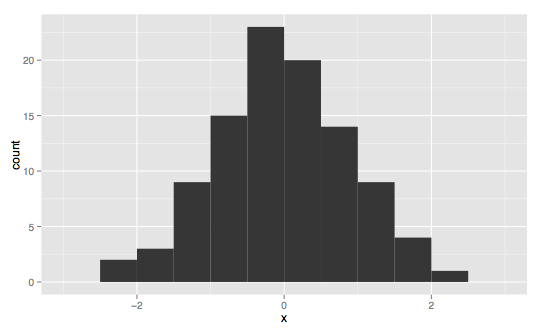
\includegraphics[height=7cm,width=12cm]{Histogram}
			\caption{A symmetric, unimodal histogram}
			\label{Histogram}
		\end{figure}

		\begin{itemize}
		\item \textbf{Remember}: histogram are for quantitative data; bar graphs are for categorical data. Also, be sure to use relative frequency histograms when comparing data sets of different sizes.
		\end{itemize}
	\end{example}

	\begin{example}[Dotplot]\index{Dotplot} \hfill \\
		
		\begin{itemize}
			\item A \textbf{Dotplot} is a representation of a distribution consists of group of data points plotted on a simple scale. Dotplots are used for continuous, quantitative, univariate data.
		\end{itemize}
	
		\begin{figure}[H]
			\centering
			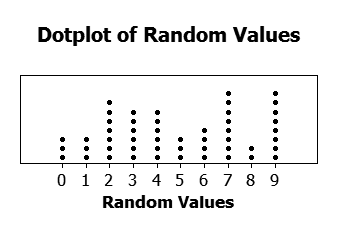
\includegraphics[height=5cm,width=7cm]{Dotplot}
			\caption{A dotplot of 50 random values from 0 to 9.}
			\label{dotplot}
		\end{figure}		
	\end{example}

	\begin{example}[Stemplot]\index{Stemplot} \hfill \\
		
		\begin{itemize}
			\item A \textbf{Stemplot} is a complicated device for presenting quantitative data in a graphical format, similar to a histogram, to assist in visualizing the shape of a distribution.
		\end{itemize}
		\begin{figure}[H]
			\centering
			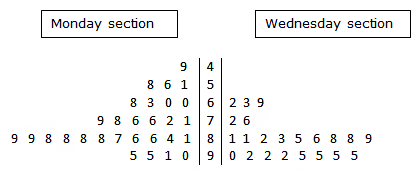
\includegraphics[height=4.4cm,width=10cm]{BTBStemplot}
			\caption{A back-to-back stemplot}
			\label{stemplot}
		\end{figure}
	\end{example}
	\newpage
	%-=-=-=-=-=-=-=-=-=-=-=-=-=-=-=-=-=-=-=-=-=-=-=-=
	%	SECTION:
	%-=-=-=-=-=-=-=-=-=-=-=-=-=-=-=-=-=-=-=-=-=-=-=-=
	
	\section{Describing Quantitative Data with Numbers}\index{Describing Quantitative Data with Numbers}
	
	\begin{exercise}[Mean and median]\index{Mean and median} \hfill \\
		
		\begin{itemize}
			\item The \textbf{Mean} is the arithmetic average of a set of number.
			\begin{definition}[Mean]\index{Mean}				
				\begin{subequations}
					\begin{align}
					\bar{x}=\frac{\text{sum of observations}}{n}=\frac{x_{1}+x_{2}+\cdot +x_{n}}{n}=\frac{\sum x_{i}}{n}
					\end{align}
				\end{subequations}
			\end{definition} \hfill
			
			\item The \textbf{Median} is the midpoint of a distribution, the number such that half the observations are smaller and half are larger.\\
			
			\item \textbf{Remember}: the \underline{median} is a \textbf{resistant} measure if center because it is relatively unaffected by extreme observations. The \underline{mean} is \textbf{nonresistant}. Among the measures of spread, the \emph{\underline{IQR}} is \textbf{resistant}, but the \underline{standard deviation} and \underline{range} are \textbf{nonresistant}.
		\end{itemize}	
	\end{exercise}
	
	\begin{exercise}[Measuring Spread]\index{Measuring Spread} \hfill \\
		
		\begin{itemize}
			\item \textbf{Interquartile range} (IQR)
			\begin{definition}[Interquartile range (IQR)]\index{Interquartile range (IQR)}			
				\begin{subequations}
					\begin{align}
					IQR=Q_{3}-Q_{1}
					\end{align}
				\end{subequations}
			\end{definition}\hfill
		
			\item \textbf{The five-number summary}			
				\begin{subequations}
					\begin{align}
					\text{The five-number summary}
						\begin{cases}
							\text{Minimum}\\
							\text{$Q_{1}$}\Longrightarrow \text{The 	\textbf{first quartile}}\\
							\text{Median}\\
							\text{$Q_{3}$}\Longrightarrow \text{The \textbf{third quartile}}\\
							\text{Maximun}
						\end{cases}
					\end{align}
				\end{subequations}\hfill 
				
			\item \textbf{Outliers}
			\begin{definition}[Outlier]\index{Outlier}
				\begin{subequations}
					\begin{align}
					\text{Outlier}
						\begin{cases}
						>Q_{3}+(1.5\times IQR)\\
						<Q_{1}-(1.5\times IQR)
						\end{cases}
					\end{align}
				\end{subequations}
				\end{definition}\hfill \\ \hfill \\ \hfill \\ \hfill \\ \hfill \\
				
			\item \textbf{Standard Deviation}  $s_{x}$ measures the typical distance of the values in  a distribution from the mean.
			\begin{definition}[Standard Deviation]\index{Standard Deviation}			
				\begin{subequations}
					\begin{align}
					S_{x}=\sqrt{\frac{1}{n-1}\sum(x_{i}-\bar{x})^{2}}
					\end{align}
				\end{subequations}
			\end{definition}\hfill
				
			\item \textbf{Variance} $s^{2}_{x}$  is the average squared deviation of a set of number.
			\begin{definition}[Variance]\index{Variance}			
				\begin{subequations}
					\begin{align}
					S^{2}_{x}=\frac{(x_{1}-\bar{x})^{2}+(x_{2}-\bar{x})^{2}+\cdots+(x_{n}-\bar{x})^{2}}{n-1}=\frac{1}{n-1}\sum(x_{i}-\bar{x})^{2}
					\end{align}
				\end{subequations}
			\end{definition}\hfill
				
			\item \textbf{Remember}: The \underline{mean} and \underline{standard deviation} are good descriptions for roughly \textbf{symmetric} distributions without outliers. The \underline{median} and \underline{\emph{IQR}} are a better description for \textbf{skewed} distributions.
					
		\end{itemize}
	\end{exercise}	
\end{document}